\section{Supplementary methods and diagnostics}
\label{app:details}

\subsection{Configuration details}
\label{app:conf-details}

The experiments share a base training configuration with per-model settings. Table~\ref{tab:app-config} lists the resolved settings for the main Hydrostatic FNO. The direct baselines and the cross-resolution and windowed variants reuse the same training procedure and differ only in their architecture- or task-specific settings.

\begin{table}[pos=htbp]
\centering
\caption{Key resolved settings for the main Hydrostatic FNO. Output channels equal the number of predicted frames times the per-frame channel count.}
\label{tab:app-config}
\begin{tabular}{lll}
    \toprule
    Group & Setting & Value \\
    \midrule
    Architecture & spectral modes ($m_1, m_2$) & $14,\,14$ \\
                 & width / depth & $48$ / $6$ \\
                 & spatial padding & $6$ \\
                 & coordinate grid channels & enabled \\
    \midrule
    Optimization & optimizer & AdamW \\
                 & learning rate / minimum & $5\times10^{-4}$ / $5\times10^{-5}$ \\
                 & schedule & cosine \\
                 & weight decay / gradient clip & $10^{-6}$ / $1.0$ \\
                 & loss & horizon-weighted MSE \\
                 & weight range / power & $0.8$--$2.0$ / $1.7$ \\
                 & maximum epochs / patience & $256$ / $20$ \\
                 & checkpoint metric & validation relative $L_2$ \\
    \midrule
    Data         & train / validation / test pools & $10{,}000$ / $1{,}000$ / $2{,}500$ \\
    Direct models & selected training seed & $18$ \\
    Ensemble     & member seeds & $\{11,22,33,44,55,66,77\}$ \\
    \bottomrule
\end{tabular}
\end{table}

\subsection{Archival training-time summary}
\label{app:training-time}

To document computational cost, Table~\ref{tab:app-training-time} summarizes wall-clock time for the two conditional windowed models. These are archival measurements from shared university-cluster jobs rather than a controlled efficiency comparison. Each completed run used a maximum of $256$ epochs, and the reported totals include restart attempts.

\begin{table}[pos=htbp]
\centering
\caption{Archival wall-clock training time for the conditional windowed models. Values are in hours except for the final column. Means are across three training seeds. The F-FNO Window-5 seed-$67$ value is a range because the logs do not contain the timing of the initial epochs before the epoch-$97$ checkpoint.}
\label{tab:app-training-time}
\small
\begin{tabular}{lccccc}
    \toprule
    Model & seed $18$ & seed $36$ & seed $67$ & mean wall time & mean s/epoch \\
    \midrule
    Window-FNO-5 & $22.38$ & $30.44$ & $30.46$ & $27.76 \pm 4.66$ & $390.4 \pm 65.5$ \\
    Window-F-FNO-5 & $32.66$ & $26.38$ & $25.34$--$28.57 ^ {\dagger}$ & $28.13$--$29.20 ^ {\dagger}$ & $395.5$--$410.7^{\dagger}$ \\
    \bottomrule
\end{tabular}

\vspace{0.35em}
\begin{minipage}{0.94\linewidth}
\footnotesize
\textsuperscript{\(\dagger\)} The seed-$67$ F-FNO record contains a checkpointed continuation: $5.42$ hours on the initial A100 attempt and $11.97$ hours on the subsequent L40 attempt are directly observed. The unlogged epochs $0$--$96$ are estimated from the successful continuation rate and the two complete peer-seed runs; the resulting range is retained rather than presented as an exact duration.
\end{minipage}
\end{table}

\subsection{Supplementary numerical evidence}
\label{app:validation-details}

The numerical evidence combines current R6 checks with earlier numerical-method and independent-comparator studies. Table~\ref{tab:app-validation-chain} expands the summary in Table~\ref{tab:solver-validation}; the current checks re-audited all train, validation, and test splits of the three datasets, reran nine representative solver cases, and added a fresh three-case R6 GeoClaw SWE comparison. The broader numerical studies remain historical and separately scoped. The 50 learning targets are adjacent-natural-step common-time outputs; no solver-step-indexed output is mixed into the reported evaluation.

\begin{table}[pos=htbp]
\centering
\caption{Supplementary scope of the numerical verification and comparison evidence.}
\label{tab:app-validation-chain}
\small
\begin{tabular}{p{0.25\linewidth}p{0.49\linewidth}p{0.17\linewidth}}
    \toprule
    Evidence & Quantitative scope & Interpretation \\
    \midrule
    Current dataset and solver checks & $3$ datasets; all train/validation/test splits; $9$ representative solver cases & passed \\
    Shared inputs & $13{,}500$ scenarios reused exactly across three references & identity established \\
    Current R6 GeoClaw SWE comparison & $3$ fixed test cases; $6$ Hydrostatic/MUSCL-HR comparisons & completed diagnostic \\
    Historical internal numerical checks & $86$ cases; $48$ analytical, numerical, and stability criteria fixed before evaluation & met criteria \\
    Historical independent comparisons & $3$ primary comparisons, $2$ verification checks, and $7$ refinement checks & retained separately \\
    Historical descriptive comparison & $12$ exploratory GeoClaw/Clawpack comparisons & $11$ outside limits \\
    Historical integrated procedure checks & $90$ cases plus $3$ deterministic repeatability checks & repeatable \\
    Historical held-out sensitivity checks & $363$ paired cases and $726$ solver executions under $42$ criteria & met criteria \\
    Dataset consistency checks & $3$ representative cases; corrected $384 \rightarrow 128 \rightarrow 192 \rightarrow 64$ grid construction & passed \\
    \bottomrule
\end{tabular}
\end{table}

The current R6 GeoClaw comparison is the relevant independent-comparator evidence for the published benchmark: Hydrostatic trajectory relative $L_2$ ranges from $0.2071$ to $0.3326$, while MUSCL-HR ranges from $0.0659$ to $0.1562$, across the three fixed cases in Table~\ref{tab:geoclaw-r6}. GeoClaw receives the exact frozen $192 \times 192$ initial state, and its central $128 \times 128$ output is block-mean reduced to the published $64 \times 64$ field. The historical exploratory comparisons and ablation remain provenance for the earlier program, not a rerun of the current benchmark. The numerical program therefore supports the specific finite-horizon procedure used here, but does not establish pointwise equivalence, general boundary independence, formal convergence, or event-scale validity.

\paragraph{Boussinesq dispersion diagnostic.}
Small-amplitude periodic sinusoidal waves are propagated on a $256 \times 32$ constant-depth grid for modes $1, 2, 4, 8, 12, 16, 24, 32$ at $\Delta t = 1.25 \times 10 ^ {-4}$ and final time $1.5$. Fourier phase tracking is compared with the discrete relation
\begin{equation}
    \omega ^ 2 =
    \frac{g H k_d ^ 2}{1 + \alpha_B H ^ 2 k_d ^ 2},
    \qquad
    k_d = \frac{2 \sin(k \Delta x / 2)}{\Delta x}.
\end{equation}
The $\alpha_B = 0$ branch approaches the non-dispersive shallow-water relation, while $\alpha_B = 1/3$ slows higher modes according to the weakly dispersive operator used here. Figure~\ref{fig:app-bouss-dispersion} shows the phase-speed comparison, and Table~\ref{tab:app-bouss-dispersion} gives the maximum errors and linear-solver status. This is a local numerical diagnostic, not external-solver or event validation.

\begin{figure}[pos=htbp]
\centering

\includegraphics[width=0.7\linewidth]{figures/boussinesq_dispersion.pdf}
\caption{Constant-depth periodic Boussinesq dispersion diagnostic. Markers are phase speeds measured by Fourier phase tracking; dashed curves are the discrete relation used for comparison.}
\label{fig:app-bouss-dispersion}
\end{figure}

\begin{table}[pos=htbp]
\centering
\caption{Summary of the Boussinesq dispersion diagnostic. The $\alpha_B = 0$ branch uses a direct linear-solver path; the $\alpha_B = 1/3$ branch uses the conjugate-gradient acceleration solve.}
\label{tab:app-bouss-dispersion}
\begin{tabular}{lccc}
    \toprule
    $\alpha_B$ & modes & maximum relative error & CG status \\
    \midrule
    $0$     & $1, 2, 4, 8, 12, 16, 24, 32$ & $2.45 \times 10 ^ {-4}$ & direct path \\
    $1 / 3$ & $1, 2, 4, 8, 12, 16, 24, 32$ & $1.91 \times 10 ^ {-8}$ & all solves converged; max.\ $35$ iterations \\
    \bottomrule
\end{tabular}
\end{table}

\subsection{Additional result tables}
\label{app:add-result-tab}

\paragraph{Seed stability and ensemble calibration.}
The seven FNO members in Table~\ref{tab:app-ensemble} differ only in seed. Their held-out Hydrostatic denormalized benchmark-scale relative $L_2$ values range from $0.257$ to $0.273$ (mean $0.265$, standard deviation $0.0055$). This quantifies the stability of the uncertainty ensemble; it is not a replicated architecture comparison.

\begin{table}[pos=htbp]
\centering
\caption{Completed seven-member Hydrostatic FNO ensemble, evaluated on the common $N = 2500$ test split.}
\label{tab:app-ensemble}
\begin{tabular}{lcc}
    \toprule
    Seed & selected epoch & denormalized rel-$L_2$ \\
    \midrule
    $11$ & $140$ & $0.263$ \\
    $22$ & $132$ & $0.266$ \\
    $33$ & $162$ & $0.257$ \\
    $44$ & $94$  & $0.273$ \\
    $55$ & $98$  & $0.267$ \\
    $66$ & $68$  & $0.271$ \\
    $77$ & $118$ & $0.261$ \\
    \bottomrule
\end{tabular}
\end{table}

Figure~\ref{fig:app-ensemble-reliability} summarizes the ensemble coverage before and after scalar variance inflation, while Table~\ref{tab:app-ensemble-calibration} reports the suite-wise $90\%$ values. Raw intervals under-cover; on the ordinary test split their marginal coverages at nominal $50/80/90/95\%$ are $0.368/0.591/0.682/0.743$. A scalar variance inflation $\sigma ^ 2 \mapsto\gamma\sigma ^ 2$, fitted on validation labels only with $\gamma = 4.995$ (standard-deviation scale $2.235$), raises test $90\%$ coverage to $0.910$. The error--uncertainty correlation on the test split is $0.496$. These coverages are per-element summaries over correlated pixels and frames, so they diagnose interval scale rather than independent-sample probabilities or operational risk.

\begin{figure}[pos=htbp]
\centering

\includegraphics[width=0.74\linewidth]{figures/ensemble_reliability.pdf}
\caption{Ensemble reliability curves before and after validation-only scalar variance inflation. The correction improves marginal coverage but remains a post-hoc per-element diagnostic.}
\label{fig:app-ensemble-reliability}
\end{figure}

\begin{table}[pos=htbp]
\centering
\caption{Nominal $90\%$ marginal coverage before and after the validation-only scalar variance inflation.}
\label{tab:app-ensemble-calibration}
\begin{tabular}{lcc}
    \toprule
    Suite & raw & calibrated \\
    \midrule
    Validation & $0.688$ & $0.914$ \\
    Test & $0.682$ & $0.910$ \\
    Multi-Gaussian subset & $0.613$ & $0.877$ \\
    Trench subset & $0.697$ & $0.918$ \\
    High source-strength tail & $0.512$ & $0.796$ \\
    \bottomrule
\end{tabular}
\end{table}

\subsection{Sample-scaling diagnostic}
\label{app:sample-scaling}

The six seed-$18$ Hydrostatic FNO subset experiments in Figure~\ref{fig:sample-scaling} use the same held-out test split and training procedure; Table~\ref{tab:sample-scaling} gives the corresponding numerical values. Their test relative $L_2$ decreases monotonically from $0.544$ at $N = 100$ to $0.259$ at $N = 5{,}000$, while the $N = 10{,}000$ direct FNO reaches $0.240$. This is a diagnostic learning curve, not a fitted or multi-seed scaling law.

\begin{figure}[pos=htbp]
\centering
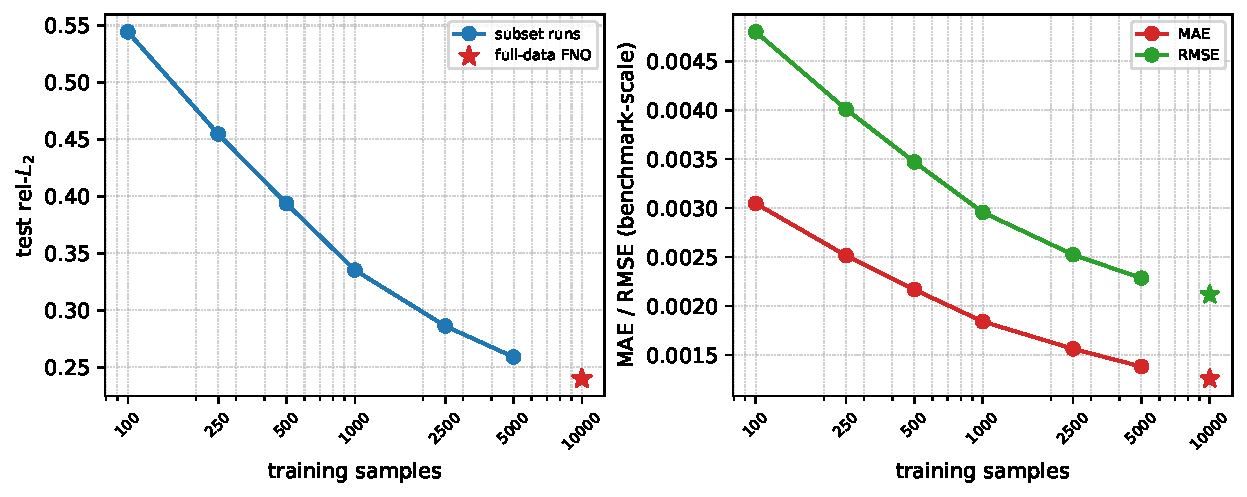
\includegraphics[width=0.94\linewidth]{figures/sample_scaling_combined.pdf}
\caption{Hydrostatic FNO sample scaling for seed-$18$ model states. Left: held-out relative-$L_2$. Right: denormalized benchmark-scale MAE and RMSE. Stars denote the full-data comparator.}
\label{fig:sample-scaling}
\end{figure}

\begin{table}[pos=htbp]
\centering
\caption{Hydrostatic FNO sample-scaling metrics on the fixed held-out test split. All rows use seed $18$. MAE and RMSE are in denormalized benchmark-scale units; maximum error is normalized.}
\label{tab:sample-scaling}
\begin{tabular}{rrcccc}
    \toprule
    Train $N$ & Seed & MAE & RMSE & rel-$L_2$ & max-err \\
    \midrule
    $100$ & $18$ & $0.00305$ & $0.00480$ & $0.544$ & $20.6$ \\
    $250$ & $18$ & $0.00251$ & $0.00401$ & $0.455$ & $16.1$ \\
    $500$ & $18$ & $0.00217$ & $0.00347$ & $0.394$ & $13.8$ \\
    $1{,}000$ & $18$ & $0.00184$ & $0.00296$ & $0.335$ & $11.9$ \\
    $2{,}500$ & $18$ & $0.00156$ & $0.00252$ & $0.286$ & $10.9$ \\
    $5{,}000$ & $18$ & $0.00138$ & $0.00228$ & $0.259$ & $11.3$ \\
    $10{,}000$ & $18$ & $0.00126$ & $0.00212$ & $0.240$ & $11.1$ \\
    \bottomrule
\end{tabular}
\end{table}

\paragraph{Conditional seeded-window diagnostics.}
The windowed models predict in $K = 5$ frame blocks after receiving the first true target frame, then are scored on the remaining $49$ frames. They solve an easier conditional rollout task than a direct 50-frame prediction and are therefore reported separately. On the ordinary Hydrostatic test split, Window-FNO-5 obtains denormalized benchmark-scale relative $L_2 = 0.031$ and Window-F-FNO-5 obtains $0.031$ (Table~\ref{tab:app-window}). The corresponding direct FNO and F-FNO values are $0.240$ and $0.230$, respectively, but the tasks are not like-for-like.

\begin{table}[pos=htbp]
\centering
\caption{Conditional seeded-window diagnostics on the $N = 2500$ Hydrostatic test split.}
\label{tab:app-window}
\begin{tabular}{lccccc}
    \toprule
    Model & predicted frames & denormalized rel-$L_2$ & MAE & RMSE & rollout time (ms) \\
    \midrule
    Window-FNO-5 & $49$ & $0.031$ & $0.000155$ & $0.000265$ & $2.65$ \\
    Window-F-FNO-5 & $49$ & $0.031$ & $0.000171$ & $0.000262$ & $4.77$ \\
    \bottomrule
\end{tabular}
\end{table}

\FloatBarrier
\subsection{Real-bathymetry diagnostics}
\label{app:real-bathymetry}

The real-bathymetry extension remains a synthetic-forcing transfer study. Table~\ref{tab:app-real-bath-window} gives the role and aggregate model errors for each suite. The ten-crop offshore morphology suite and the fully wet coastline ablation rescale bathymetry into the fully wet training range, while the wet--dry coastline stress case preserves positive topography and is outside the main training distribution. Figure~\ref{fig:app-real-bath} shows representative reference fields.

\begin{table}[pos=htbp]
\centering
\caption{Role and relative-$L_2$ metrics of the common-time real-bathymetry suites. All use synthetic forcing and Hydrostatic reference labels. Windowed columns are first-target-frame-seeded and scored on the remaining $49$ frames, so they are not like-for-like direct predictions.}
\label{tab:app-real-bath-window}
\footnotesize
\setlength{\tabcolsep}{2.5pt}
\begin{tabular}{lp{0.23\linewidth}ccccc}
    \toprule
    Suite & Role & $n$ & direct FNO & direct F-FNO & Window-FNO-5 & Window-F-FNO-5 \\
    \midrule
    Ten-crop offshore morphology & main fully wet transfer & $10$ & $0.358$ & $0.293$ & $0.066$ & $0.063$ \\
    Tohoku offshore crop & illustrative suite member & $1$ & $0.212$ & $0.235$ & $0.035$ & $0.038$ \\
    Coastline fully wet & training-range geometry ablation & $1$ & $0.245$ & $0.258$ & $0.029$ & $0.027$ \\
    Coastline wet--dry & out-of-distribution stress test & $1$ & $0.998$ & $0.997$ & $1.035$ & $1.128$ \\
    \bottomrule
\end{tabular}
\end{table}

\begin{figure}[pos=htbp]
\centering

\includegraphics[width=\linewidth]{figures/real_bathymetry_suites.pdf}
\caption{GEBCO\_2026-derived bathymetry-suite snapshots \citep{gebco2026} at the final requested time, $t = 420$ in elapsed benchmark-time units. Top: fully wet offshore morphology. Middle: coastline wet--dry stress case with positive topography retained. Bottom: the same coastline geometry rescaled into the fully wet range. These are synthetic-forcing transfer diagnostics, not real-event validation.}
\label{fig:app-real-bath}
\end{figure}

\FloatBarrier
\subsection{Selected high-error cases}
\label{app:failure-cases}

Figure~\ref{fig:app-failure-cases} intentionally selects difficult examples, not representative or average cases. The columns are an ordinary rough-source test case, a strict rough-source holdout case, and the wet--dry coastline stress case. Their full-trajectory denormalized benchmark-scale relative $L_2$ values are listed in Table~\ref{tab:app-failure-cases}. The selected examples make the failure modes visible without changing the aggregate metrics reported in the main text.

\begin{figure}[pos=htbp]
\centering

\includegraphics[width=0.73\linewidth]{figures/appendix_failure_cases.pdf}
\caption{Selected high-error cases, not average or representative examples. Columns are the three cases; rows show denormalized bathymetry, source, late-frame Hydrostatic reference $\eta$, FNO prediction, and absolute error. The coastline stress case uses GEBCO\_2026-derived morphology \citep{gebco2026}.}
\label{fig:app-failure-cases}
\end{figure}

\begin{table}[pos=htbp]
\centering
\caption{Selected high-error examples. Values are full-trajectory denormalized benchmark-scale relative $L_2$.}
\label{tab:app-failure-cases}
\begin{tabular}{llc}
    \toprule
    Case & sample & denormalized rel-$L_2$ \\
    \midrule
    Ordinary rough-source test case & \texttt{sample\_001460} & $0.630$ \\
    Strict rough-source holdout & \texttt{sample\_000713} & $0.718$ \\
    Coastline wet--dry stress case & \texttt{sample\_000001} & $0.998$ \\
    \bottomrule
\end{tabular}
\end{table}
